\subsection{Standard Baseline and Adaptive Optimizers}
\paragraph{SGD with Momentum.}
\begin{figure}[H]
\centering
\fitfigure{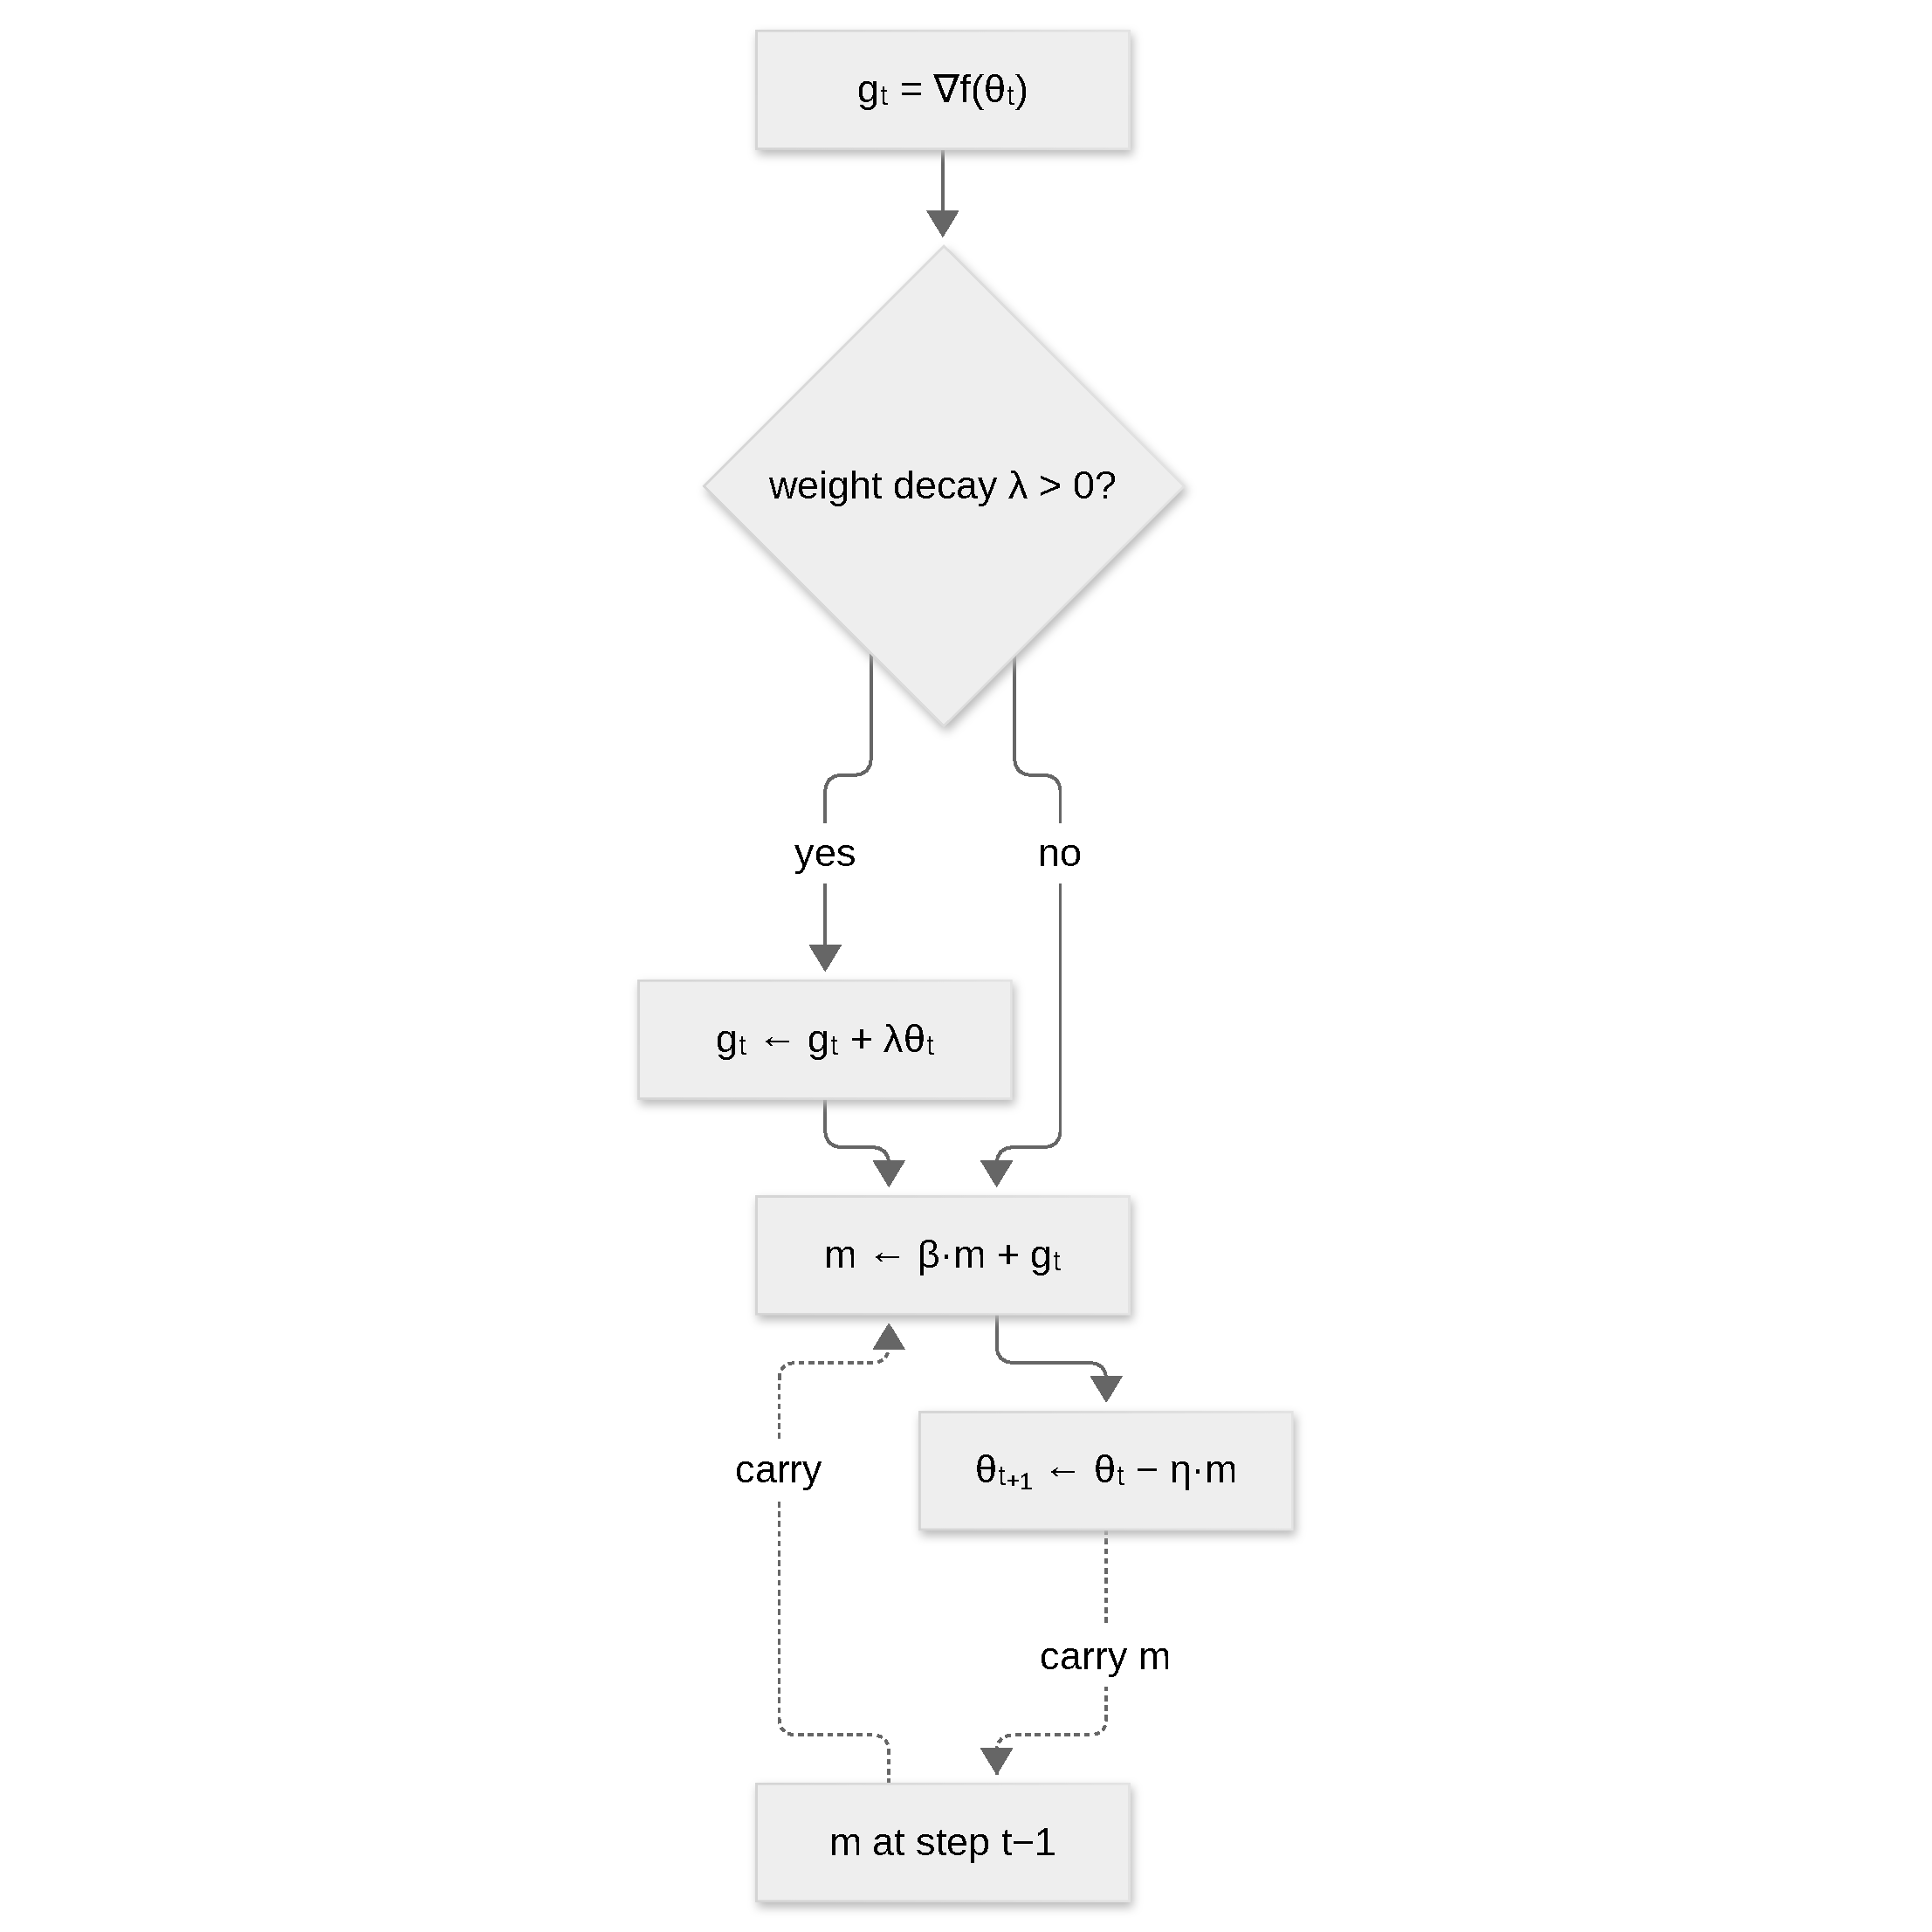
\includegraphics{figures/optimizers/sgd-momentum.pdf}}
\caption{Step flow of SGD with momentum: optional L2 weight decay, exponential momentum accumulation, and the fixed-step parameter update.}
\label{fig:opt-sgd-momentum}
\end{figure}
The classical update accumulates a momentum buffer and then applies a fixed learning rate. At each iteration $t$, the algorithm maintains an exponential moving average $m_t$ of past gradients:
\begin{align}
m_t &= \beta m_{t-1} + g_t \\
\theta_{t+1} &= \theta_t - \eta m_t
\end{align}
where $g_t = \nabla f(\theta_t)$, $\beta \in [0.8, 0.99]$ controls the momentum decay, and $\eta$ is the fixed learning rate. The momentum term acts as velocity: it accelerates movement in consistent directions while dampening oscillations in variable directions.

\begin{algorithm}[H]
\caption{SGD with Momentum}
\label{alg:sgd-momentum}
\begin{algorithmic}[1]
\Require Initial parameters $\theta_0$, learning rate $\eta$, momentum coefficient $\beta$, weight decay $\lambda$
\Ensure Updated parameters $\theta_T$
\State Initialize: momentum buffer $m \gets 0$
\For{$t = 0, 1, 2, \ldots, T-1$}
    \State Compute gradient: $g_t \gets \nabla f(\theta_t)$
    \If{weight\_decay $> 0$}
        \State $g_t \gets g_t + \lambda \theta_t$ \Comment{L2 regularization}
    \EndIf
    \State Update momentum: $m \gets \beta \cdot m + g_t$
    \State Update parameters: $\theta_{t+1} \gets \theta_t - \eta \cdot m$
\EndFor
\Return $\theta_T$
\end{algorithmic}
\end{algorithm}

\paragraph{Cons.}
\begin{itemize}[leftmargin=*]
\item Poor robustness to heterogeneous curvature: a single global rate cannot suit every parameter group.
\item Strong dependence on carefully engineered learning-rate schedules.
\end{itemize}

\paragraph{Pros.}
\begin{itemize}[leftmargin=*]
\item Low memory overhead: a single momentum buffer per parameter.
\item Strong generalization when tuned carefully, and a simple update to implement.
\end{itemize}

\paragraph{Adam and AdamW.}
\begin{figure}[H]
\centering
\fitfigure{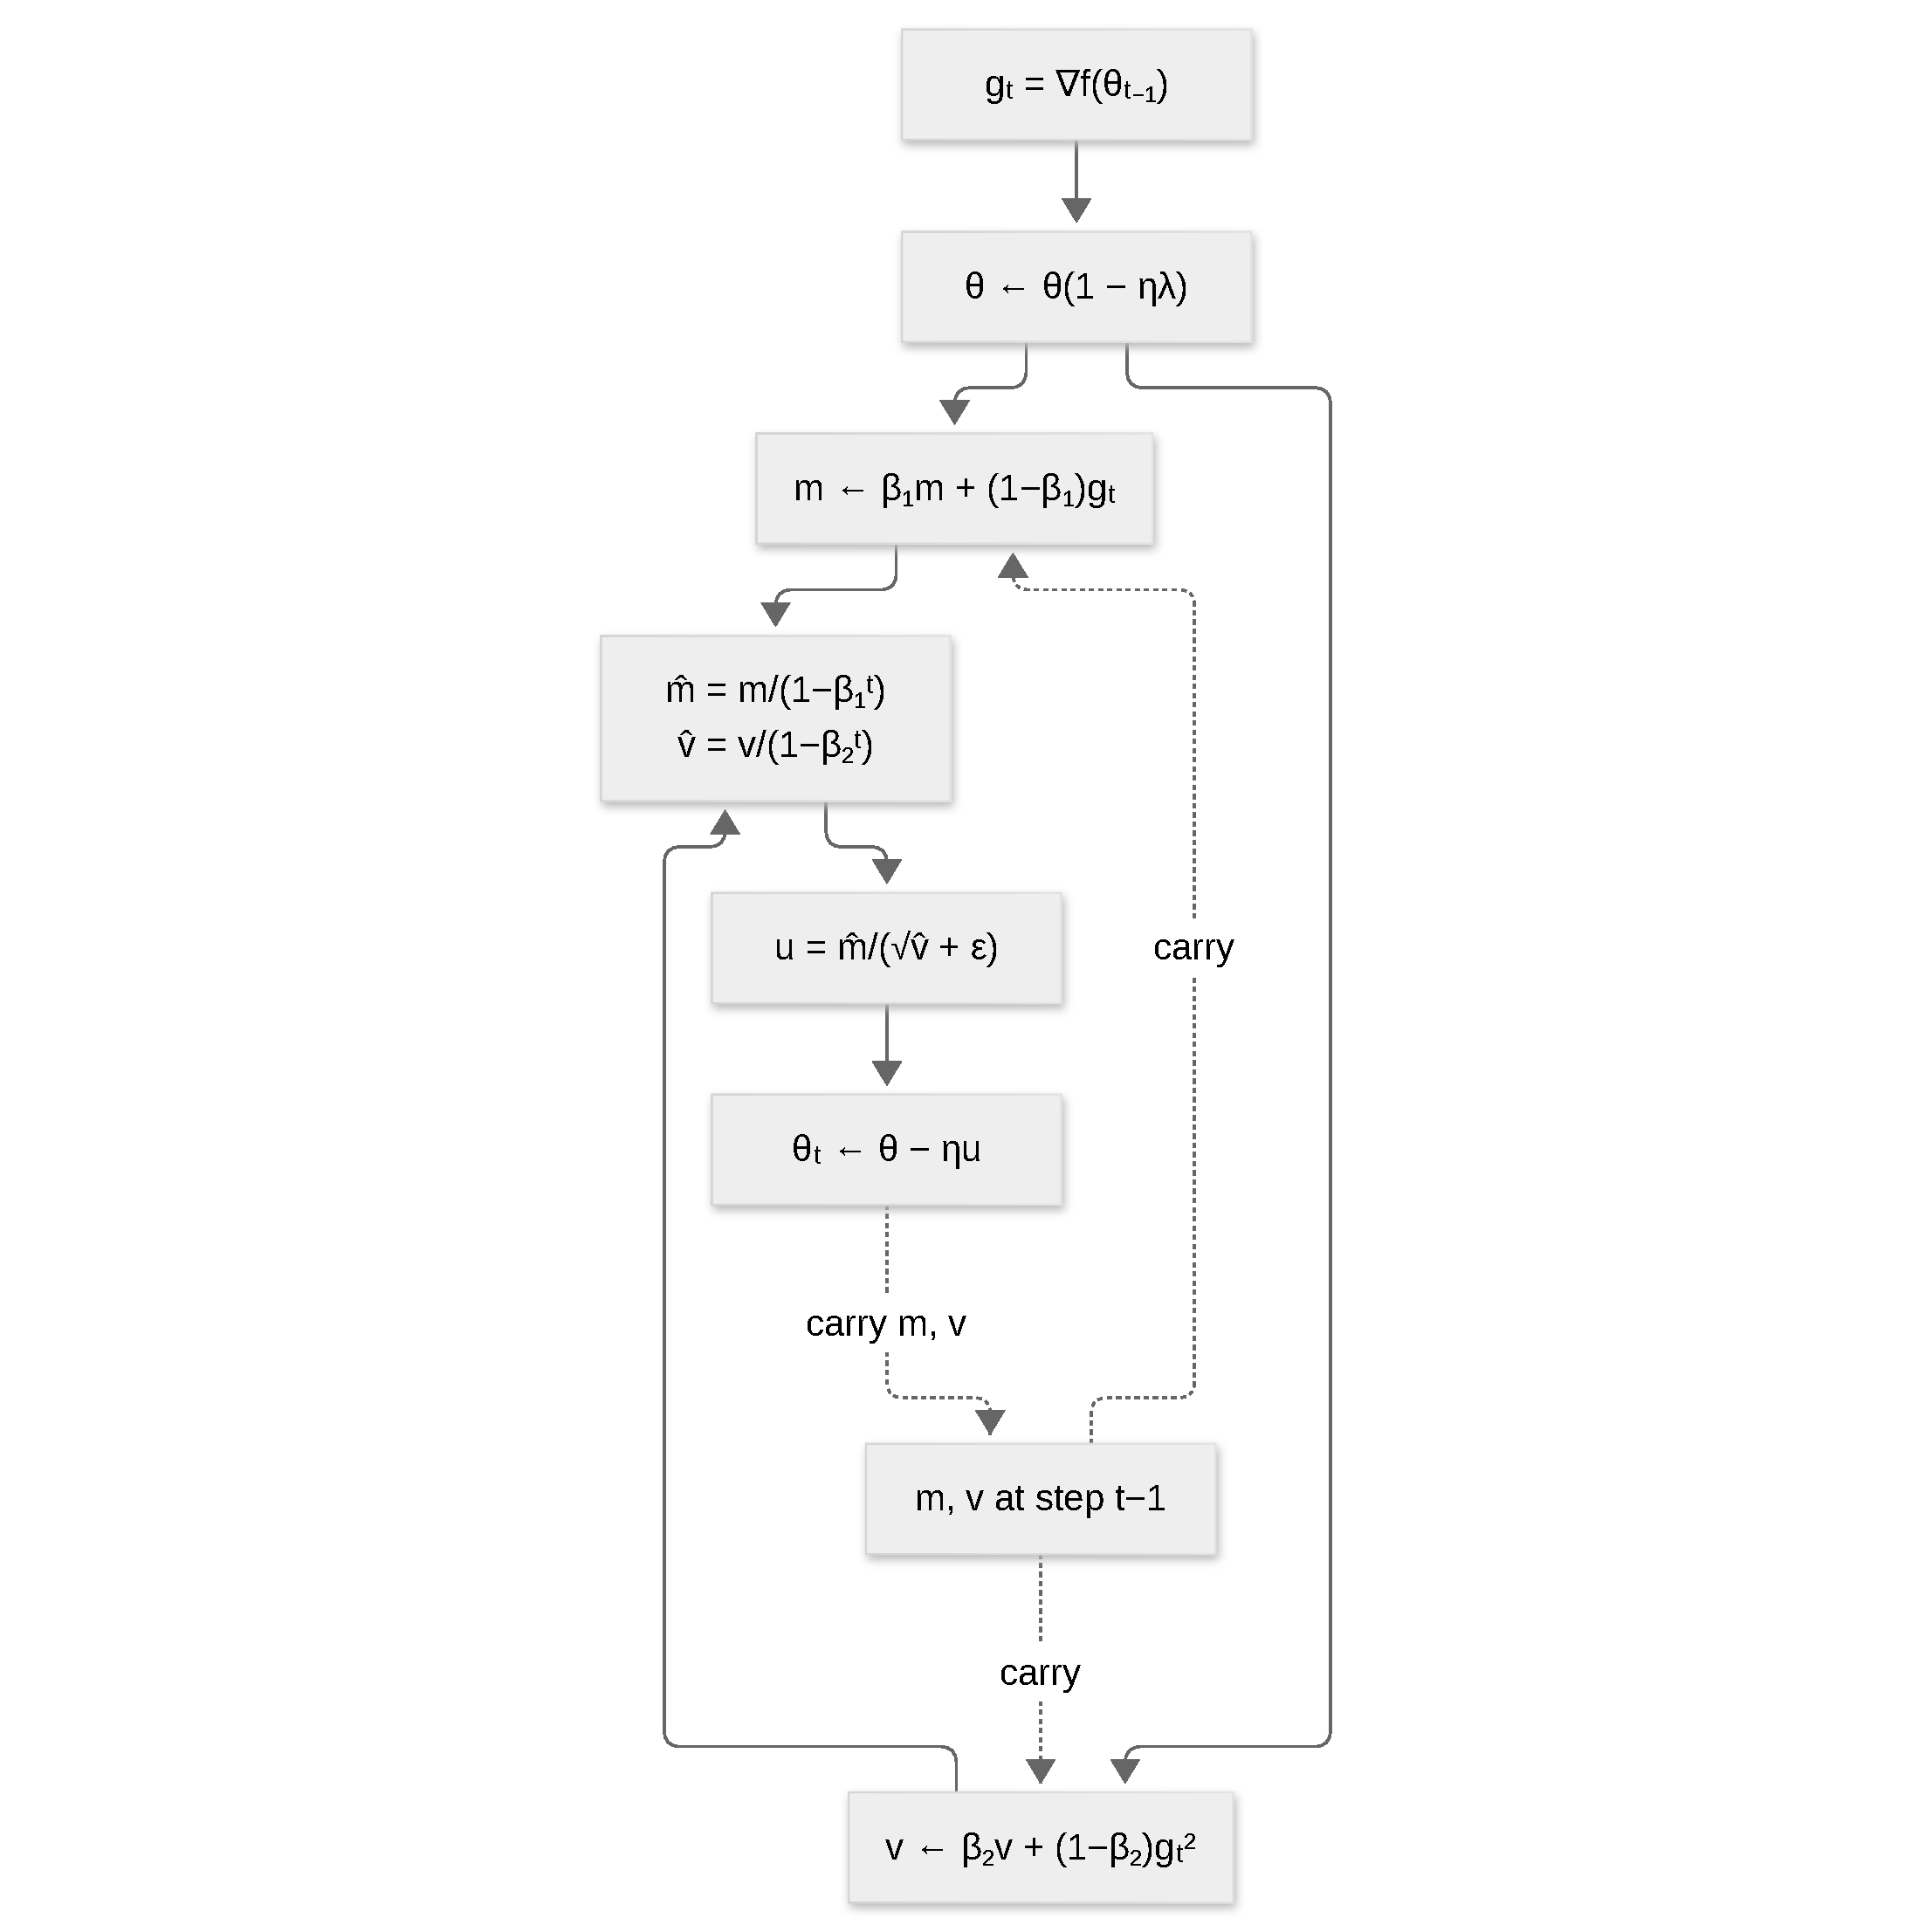
\includegraphics{figures/optimizers/adamw.pdf}}
\caption{Step flow of AdamW: decoupled weight decay, first- and second-moment EMAs, bias correction, and the element-wise adaptive update.}
\label{fig:opt-adamw}
\end{figure}
Adam tracks exponential moving averages of both first moment (mean) and second moment (uncentered variance) to achieve element-wise adaptive learning rates. The update rule is:
\begin{align}
m_t &= \beta_1 m_{t-1} + (1-\beta_1) g_t \\
v_t &= \beta_2 v_{t-1} + (1-\beta_2) g_t^2 \\
\hat{m}_t &= \frac{m_t}{1-\beta_1^t}, \quad \hat{v}_t = \frac{v_t}{1-\beta_2^t} \quad \text{(bias correction)} \\
\theta_{t+1} &= \theta_t - \eta \left(\frac{\hat{m}_t}{\sqrt{\hat{v}_t}+\epsilon}\right)
\end{align}
AdamW introduces a crucial modification: weight decay is applied directly to parameters (decoupled from gradients): $\theta_t \gets \theta_t(1-\eta\lambda)$ rather than adding $\lambda\theta_t$ to the gradient. This decoupling prevents the adaptive scaling from interfering with regularization strength.

\begin{algorithm}[H]
\caption{AdamW (Adam with Decoupled Weight Decay)}
\label{alg:adamw}
\begin{algorithmic}[1]
\Require Initial parameters $\theta_0$, learning rate $\eta$, exponential decay rates $\beta_1, \beta_2 \in [0,1)$
\Require Momentum constant $\epsilon$, weight decay $\lambda$
\Ensure Updated parameters $\theta_T$
\State Initialize: first moment $m \gets 0$, second moment $v \gets 0$, step counter $t \gets 0$
\For{$t = 1, 2, \ldots, T$}
    \State Compute gradient: $g_t \gets \nabla f(\theta_{t-1})$
    \State Weight decay (decoupled): $\theta_{t-1} \gets \theta_{t-1}(1 - \eta\lambda)$
    \State Update moments: $m \gets \beta_1 m + (1-\beta_1) g_t$
    \State $v \gets \beta_2 v + (1-\beta_2) g_t^2$
    \State Bias correction: $\hat{m} \gets m / (1 - \beta_1^t)$, $\hat{v} \gets v / (1 - \beta_2^t)$
    \State Update parameters: $\theta_t \gets \theta_{t-1} - \eta (\hat{m} / (\sqrt{\hat{v}} + \epsilon))$
\EndFor
\Return $\theta_T$
\end{algorithmic}
\end{algorithm}

\paragraph{Cons.}
\begin{itemize}[leftmargin=*]
\item Stores first and second moment tensors for every parameter, doubling optimizer-state memory relative to SGD.
\item Element-wise adaptive scaling can interfere with regularization unless weight decay is decoupled.
\end{itemize}

\paragraph{Pros.}
\begin{itemize}[leftmargin=*]
\item Practical baseline for transformer fine-tuning: fast convergence and forgiving to hyperparameter variation.
\item Decoupled weight decay keeps the regularization strength independent of the adaptive scaling.
\end{itemize}

\paragraph{RAdam (Rectified Adam).}
\begin{figure}[H]
\centering
\fitfigure{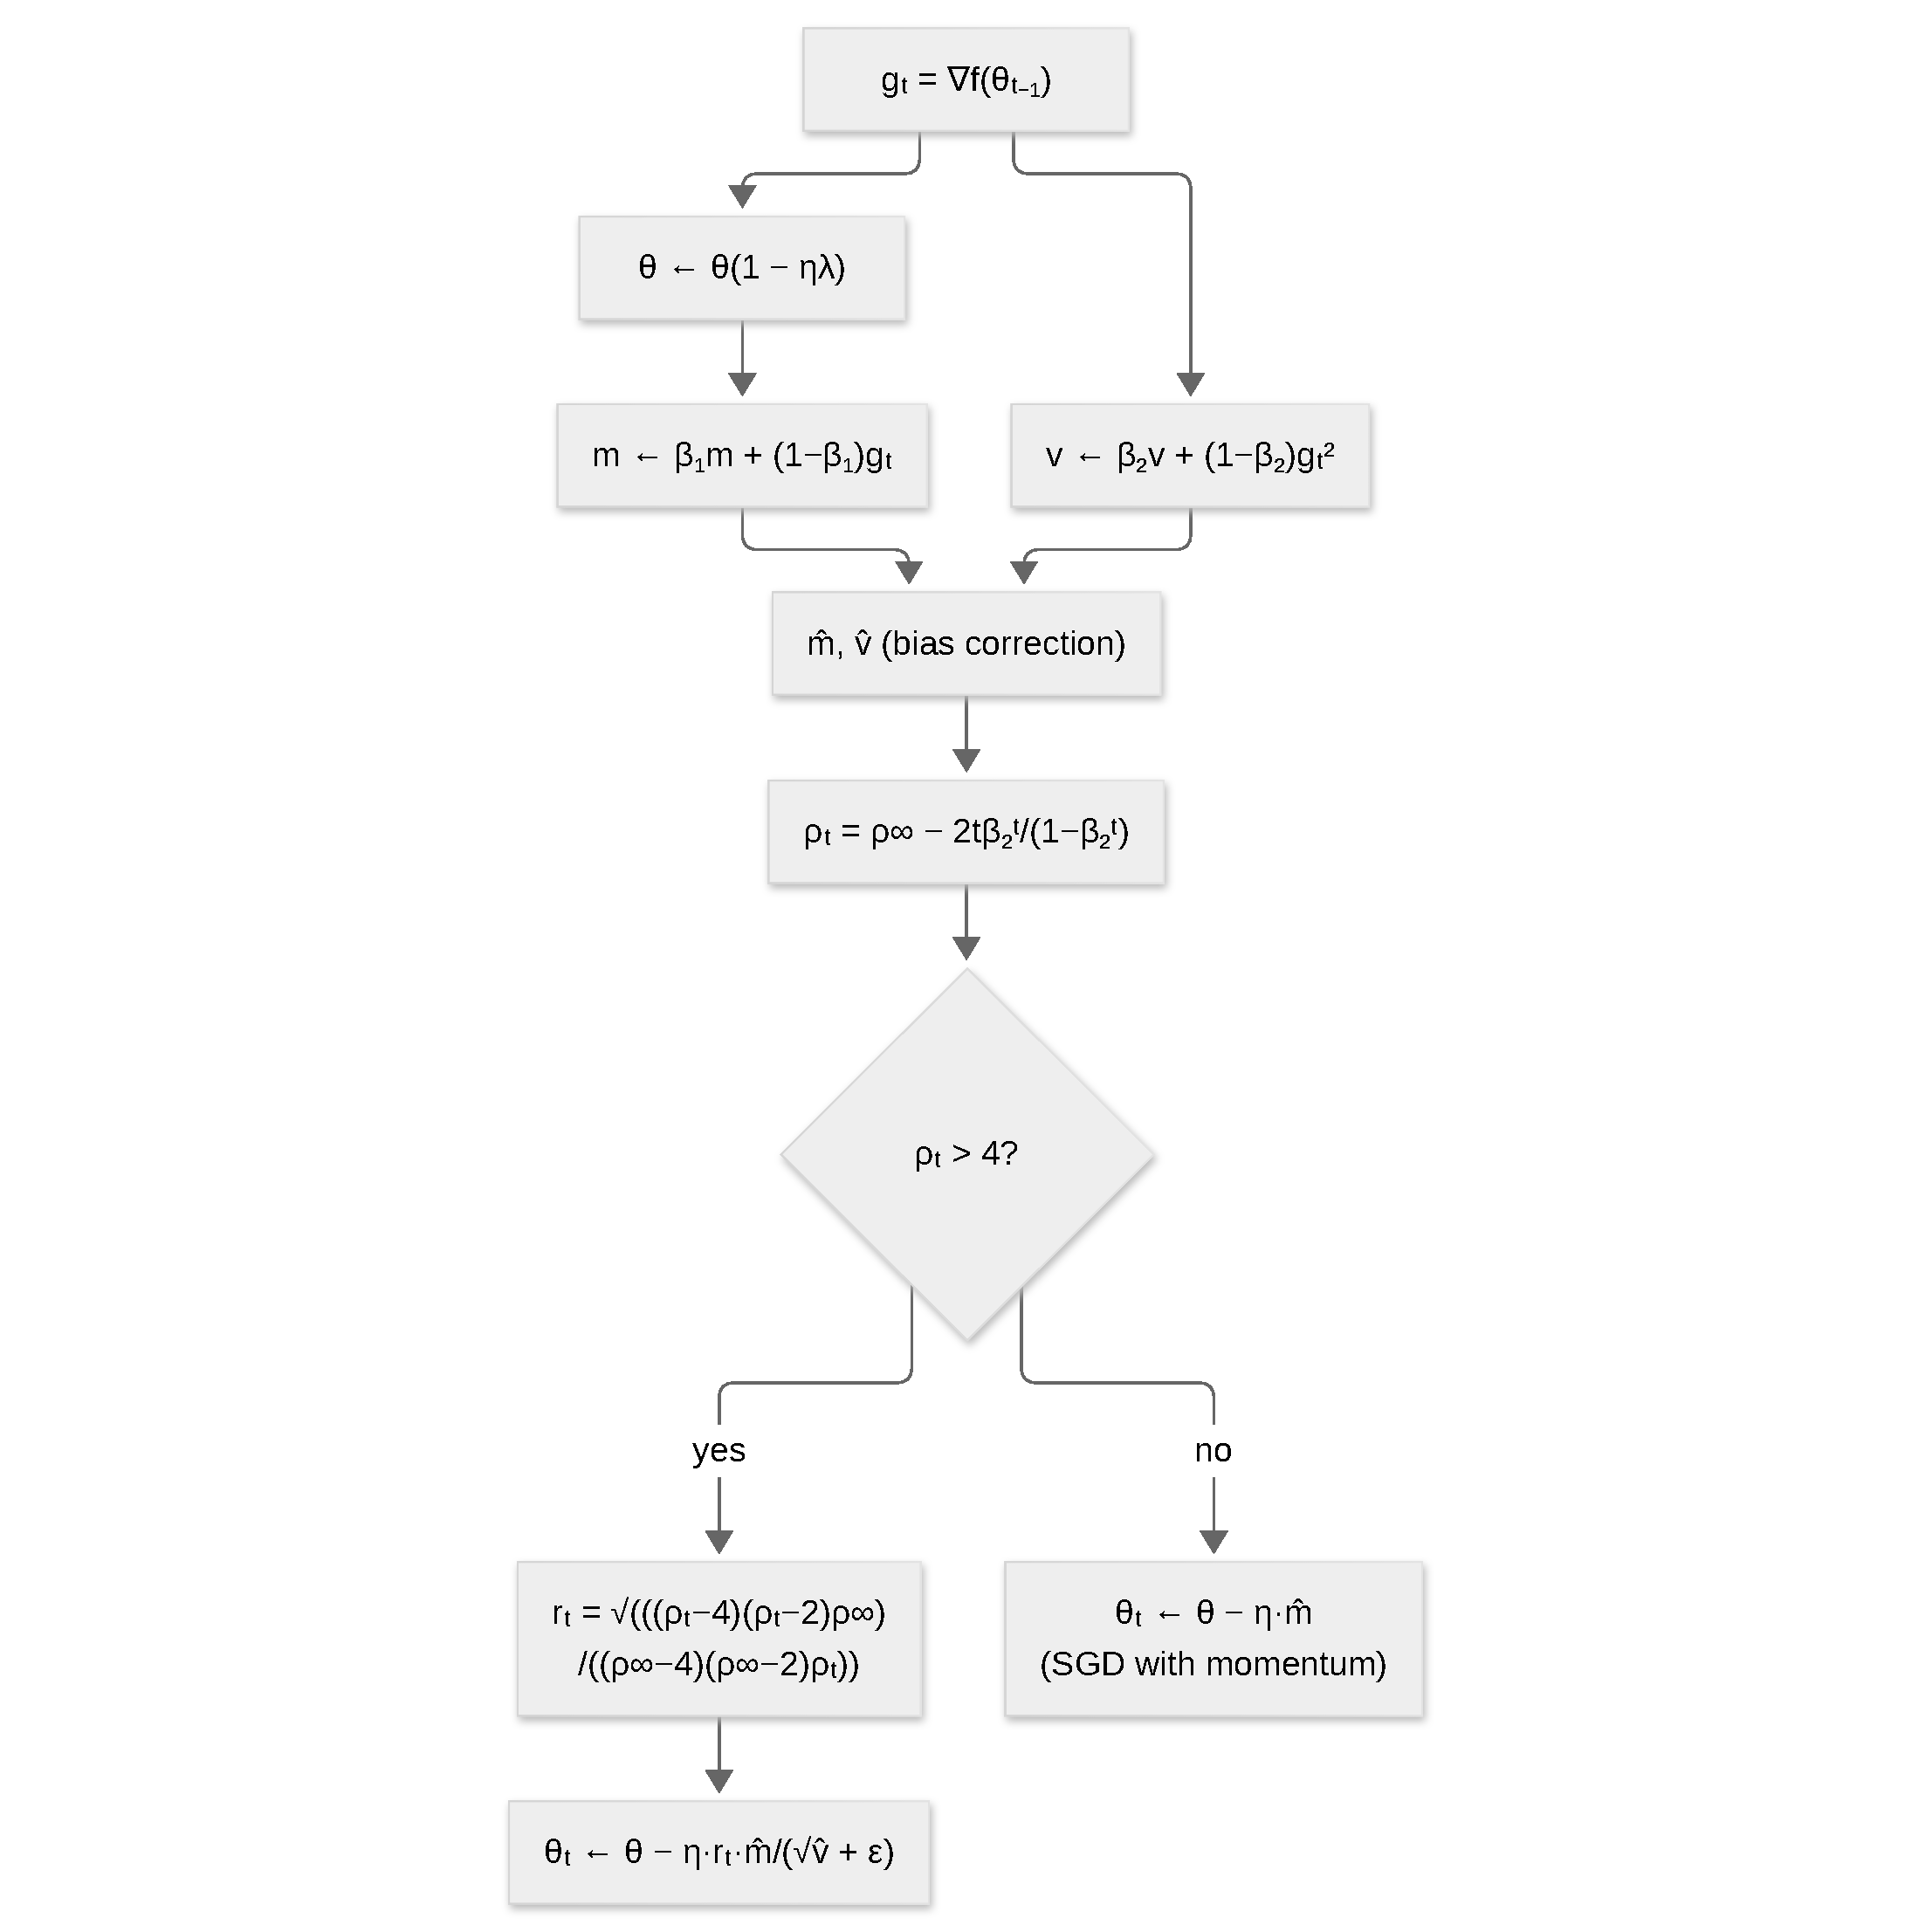
\includegraphics{figures/optimizers/radam.pdf}}
\caption{Step flow of RAdam: SMA-window rectification with an early-step fallback to momentum SGD.}
\label{fig:opt-radam}
\end{figure}
RAdam addresses Adam's instability in early training by dynamically rectifying the adaptive learning rate. The key observation is that the second moment $v_t$ has very high variance in the first few steps, causing unreliable adaptive scaling. RAdam computes the effective simple moving average (SMA) window length:
\[\rho_t = \rho_{\infty} - \frac{2t\beta_2^t}{1-\beta_2^t}, \quad \text{where} \quad \rho_{\infty} = \frac{2}{1-\beta_2}-1\]
When $\rho_t > 4$ (sufficient samples for variance estimation), RAdam applies adaptive scaling with a rectification term:
\[r_t = \sqrt{\frac{(\rho_t-4)(\rho_t-2)\rho_{\infty}}{(\rho_{\infty}-4)(\rho_{\infty}-2)\rho_t}}, \quad \theta_{t+1} = \theta_t - \eta r_t \frac{\hat{m}_t}{\sqrt{\hat{v}_t}+\epsilon}\]
When $\rho_t \leq 4$, RAdam falls back to SGD with momentum: $\theta_{t+1} = \theta_t - \eta\hat{m}_t$.

\begin{algorithm}[H]
\caption{RAdam (Rectified Adam)}
\label{alg:radam}
\begin{algorithmic}[1]
\Require Initial parameters $\theta_0$, learning rate $\eta$, $\beta_1, \beta_2$, weight decay $\lambda$
\Ensure Updated parameters $\theta_T$
\State Initialize: $m \gets 0$, $v \gets 0$, $t \gets 0$
\State Compute: $\rho_\infty \gets 2/(1-\beta_2) - 1$
\For{$t = 1, 2, \ldots, T$}
    \State $g_t \gets \nabla f(\theta_{t-1})$
    \If{weight\_decay $> 0$}
        \State $\theta_{t-1} \gets \theta_{t-1}(1 - \eta\lambda)$
    \EndIf
    \State $m \gets \beta_1 m + (1-\beta_1) g_t$
    \State $v \gets \beta_2 v + (1-\beta_2) g_t^2$
    \State $\hat{m} \gets m/(1-\beta_1^t)$, $\hat{v} \gets v/(1-\beta_2^t)$
    \State $\rho_t \gets \rho_\infty - 2t \beta_2^t / (1 - \beta_2^t)$
    \If{$\rho_t > 4$}
        \State $r_t \gets \sqrt{((\rho_t-4)(\rho_t-2)\rho_\infty) / ((\rho_\infty-4)(\rho_\infty-2)\rho_t)}$
        \State $\theta_t \gets \theta_{t-1} - \eta r_t \hat{m} / (\sqrt{\hat{v}} + \epsilon)$
    \Else
        \State $\theta_t \gets \theta_{t-1} - \eta \hat{m}$ \Comment{SGD with momentum}
    \EndIf
\EndFor
\Return $\theta_T$
\end{algorithmic}
\end{algorithm}

\paragraph{Cons.}
\begin{itemize}[leftmargin=*]
\item Adds rectification bookkeeping on top of Adam's moment state.
\item The benefit shrinks when a well-tuned warmup schedule is already in use.
\end{itemize}

\paragraph{Pros.}
\begin{itemize}[leftmargin=*]
\item Eliminates the need for manual learning-rate warmup by rectifying the adaptive rate.
\item Falls back gracefully to momentum SGD while variance estimates are unreliable, improving robustness.
\end{itemize}

